\subsection{4. Отношение эквивалентности и классификация множеств}

\subsubsection{4.1. Что такое отношение эквивалентности?}

Отношение $R$ на множестве $A$ связывает между собой некоторые пары элементов.  
Мы называем его \emph{отношением эквивалентности}, если оно позволяет считать связанные элементы «равными» по какому‑то признаку.  

Формально $R\subseteq A\times A$ удовлетворяет трём ключевым свойствам:

\begin{enumerate}[label=\arabic*)]
  \item \textbf{Рефлексивность.}  
    Каждый элемент эквивалентен сам себе:
    \[
      \forall a\in A\quad (a,a)\in R.
    \]
    \emph{Пояснение:} это значит, что сравнивая элемент с самим собой, мы всегда получаем «да» — элемент всегда «равен» самому себе.

  \item \textbf{Симметричность.}  
    Если $a$ эквивалентен $b$, то и $b$ эквивалентен $a$:
    \[
      \forall a,b\in A\;\bigl((a,b)\in R \;\Rightarrow\; (b,a)\in R\bigr).
    \]
    \emph{Пояснение:} эквивалентность — взаимное отношение. Нельзя иметь «одностороннюю» равенство.

  \item \textbf{Транзитивность.}  
    Если $a$ эквивалентен $b$, а $b$ эквивалентен $c$, то $a$ эквивалентен $c$:
    \[
      \forall a,b,c\in A\;\bigl((a,b)\in R \wedge (b,c)\in R\bigr) \;\Rightarrow\; (a,c)\in R.
    \]
    \emph{Пояснение:} признак эквивалентности «передаётся» по цепочке.
\end{enumerate}

Без одного из этих свойств отношение нельзя назвать «эквивалентностью», потому что нарушится идея «равности» как симметричной и непротиворечивой связи.

\subsubsection{4.2. Классы эквивалентности: интуитивный смысл}

\paragraph{Идея.} Все элементы, которые попарно эквивалентны друг другу, можно «собрать в одну корзинку» — \emph{класс эквивалентности}.  

Для каждого $a\in A$ определим
\[
  [a] \;=\; \{\,x\in A \mid (a,x)\in R\}.
\]
\begin{itemize}[leftmargin=*]
  \item Если $b\in[a]$, то по симметричности и транзитивности получаем $[b]=[a]$.
  \item Если два класса не совпадают, то они не имеют общих элементов:
    \[
      [a]\neq[b]\;\Longrightarrow\;[a]\cap[b]=\varnothing.
    \]
\end{itemize}

Таким образом, классы эквивалентности \emph{разбивают} всё множество $A$ на непересекающиеся «группы равных элементов».

\subsubsection{4.3. Фактор‑множество и фактор‑отображение}

Обозначим множество всех таких классов:
\[
  A/R \;=\; \{\, [a] \mid a\in A\}.
\]
Это называется \emph{фактор‑множеством}.  
С ним связано естественное отображение
\[
  \pi: A \;\longrightarrow\; A/R,\qquad
  \pi(a) = [a].
\]
\begin{itemize}[leftmargin=*]
  \item $\pi$ «сводит» каждый элемент в его класс.
  \item $\pi$ является сюръекцией (покрывает все классы).
  \item Если $aRb$, то $\pi(a)=\pi(b)$, и наоборот.
\end{itemize}

\subsubsection{4.4. Развёрнутые примеры}

\begin{enumerate}[label=\arabic*)]
  \item \textbf{Конгруэнция по модулю $n$} на $\mathbb{Z}$.  
    Определение: 
    \[
      a \equiv b \pmod{n}
      \quad\Longleftrightarrow\quad
      n \mid (a-b).
    \]
    Проверим свойства:
    \begin{itemize}[leftmargin=*]
      \item Рефлексивность: $n\mid(a-a)=0$ всегда.
      \item Симметричность: если $n\mid(a-b)$, то $n\mid(b-a)$.
      \item Транзитивность: $n\mid(a-b)$ и $n\mid(b-c)$ даёт $n\mid(a-c)$.
    \end{itemize}
    Класс $[a]=\{a+kn \mid k\in\mathbb{Z}\}$.  
    Всего $n$ различных классов: $[0], [1],\dots,[n-1]$.

  \item \textbf{Равенство длины слов} над алфавитом $\Sigma$.  
    Правило: $u\sim v \iff |u|=|v|$.  
    \begin{itemize}[leftmargin=*]
      \item Все слова длины 3 формируют один класс $[u]$.
      \item В фактор‑множестве $\Sigma^*/{\sim}$ каждый класс соответствует конкретной длине.
    \end{itemize}

  \item \textbf{Цвет точек на плоскости.}  
    Определим отношение: две точки эквивалентны, если они имеют одинаковый цвет.  
    Тогда каждый цвет — это один класс; фактор‑множество — набор всех цветов.
\end{enumerate}

\subsubsection{4.5. Геометрическая иллюстрация}

\begin{center}
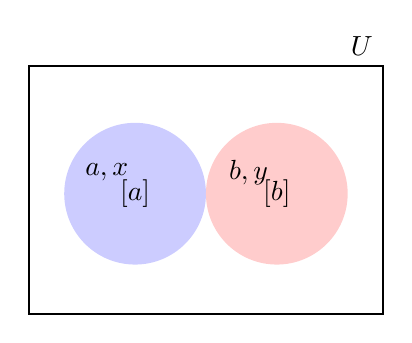
\begin{tikzpicture}[scale=0.9]
  % универсум U
  \draw[thick] (-0.5,-0.5) rectangle (4.5,3) node[above left]{$U$};
  % класс [a]
  \fill[blue!20] (1,1.2) circle (1cm);
  \node at (1,1.2) {$[a]$};
  % класс [b]
  \fill[red!20] (3,1.2) circle (1cm);
  \node at (3,1.2) {$[b]$};
  % примеры точек
  \node at (0.6,1.5) {$a,x$};  
  \node at (2.6,1.5) {$b,y$};
\end{tikzpicture}
\end{center}

Здесь каждый круг — класс эквивалентности, внутри него лежат все «равные» элементы.

\subsubsection{4.6. Зачем это нужно?}

\begin{itemize}[leftmargin=*]
  \item Упрощает работу: вместо множества элементов оперируем множеством классов.
  \item В алгебре: фактор‑группы, фактор‑кольца.
  \item В теории языков: выделение всех слов одинаковой длины, одинакового суффикса и т.\,д.
  \item В анализе данных: кластеризация, когда каждый кластер — класс эквивалентности по выбранному критерию.
\end{itemize}

\subsubsection{Источники и литература}

\begin{itemize}
  \item Г.\,С. Михалев, \emph{Дискретная математика. Базовый курс для вузов}.
  \item Р. Джонсонбауг, \emph{Дискретная математика}, Pearson Education.
  \item В.\,Э. Пахомов, \emph{Введение в дискретную математику}.
  \item \href{https://ru.wikipedia.org/wiki/Класс_эквивалентности}{Википедия: Класс эквивалентности}
  \item \href{https://ru.wikipedia.org/wiki/Фактор-множество}{Википедия: Фактор‑множество}
\end{itemize}